\documentclass[border=7pt]{standalone}
\usepackage{tikz}
\begin{document}
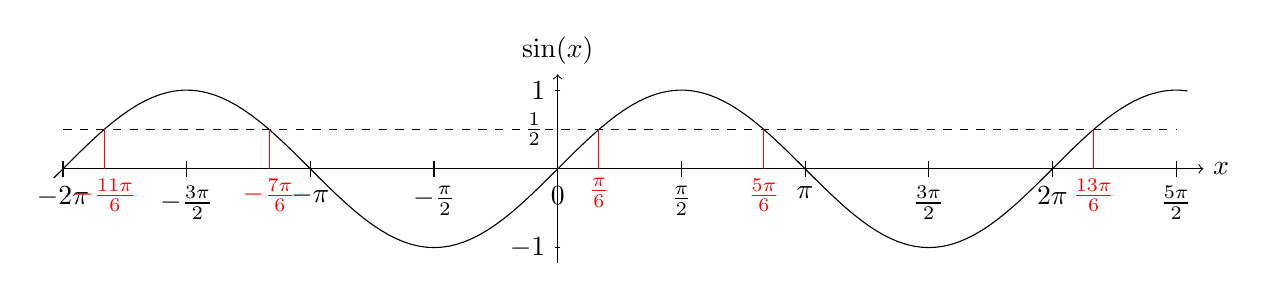
\begin{tikzpicture}[domain=-6.4:8]
  \draw[->] (-6.3,0) -- (8.2,0) node[right] {$x$};
  \draw[->] (0,-1.2) -- (0,1.2) node[above] {$\sin(x)$};
  \draw plot [samples=150] (\x,{sin(\x r)});
  \foreach \x/\xtext in {-2*pi/-2\pi, -1.5*pi/-\frac{3\pi}{2} ,-pi/-\pi, -0.5*pi/-\frac{\pi}{2}, 0,0.5*pi/\frac{\pi}{2}, pi/\pi, 1.5*pi/\frac{3\pi}{2}, 2*pi/2\pi, 2.5*pi/\frac{5\pi}{2} }
    \draw (\x,0.1) -- (\x,-0.1) node[anchor=north] {$\xtext$};
   \foreach \y/\ytext in {-1,1}
     \draw (1pt,\y cm) -- (-1pt,\y cm) node[anchor=east] {$\ytext$};

  \node (c) at (-0.3,0.5)  {$\frac{1}{2}$};
  \draw [dashed] (-6.28,0.5) -- (7.85,0.5);

  \draw [red] (0.5235, 0.5) -- (0.5235,0) node [below] {$\frac{\pi}{6}$} ;
  \draw [red] (2.6180, 0.5) -- (2.6180,0) node [below] {$\frac{5\pi}{6}$} ;
  \draw [red] (6.8065, 0.5) -- (6.8065,0) node [below] {$\frac{13\pi}{6}$} ;
  \draw [red] (-3.665, 0.5) -- (-3.665,0) node [below] {$-\frac{7\pi}{6}$} ;
  \draw [red] (-5.7596, 0.5) -- (-5.7596,0) node [below] {$-\frac{11\pi}{6}$} ;

\end{tikzpicture}
\end{document}
